% Copyright 2004 by Till Tantau <tantau@users.sourceforge.net>.
%
% In principle, this file can be redistributed and/or modified under
% the terms of the GNU Public License, version 2.
%
% However, this file is supposed to be a template to be modified
% for your own needs. For this reason, if you use this file as a
% template and not specifically distribute it as part of a another
% package/program, I grant the extra permission to freely copy and
% modify this file as you see fit and even to delete this copyright
% notice. 

\documentclass{beamer}

% There are many different themes available for Beamer. A comprehensive
% list with examples is given here:
% http://deic.uab.es/~iblanes/beamer_gallery/index_by_theme.html
% You can uncomment the themes below if you would like to use a different
% one:
%\usetheme{AnnArbor}
%\usetheme{Antibes}
%\usetheme{Bergen}
%\usetheme{Berkeley}
%\usetheme{Berlin}
%\usetheme{Boadilla}
%\usetheme{boxes}
%\usetheme{CambridgeUS}
%\usetheme{Copenhagen}
%\usetheme{Darmstadt}
\usetheme{default}
%\usetheme{Frankfurt}
%\usetheme{Goettingen}
%\usetheme{Hannover}
%\usetheme{Ilmenau}
%\usetheme{JuanLesPins}
%\usetheme{Luebeck}
%\usetheme{Madrid}
%\usetheme{Malmoe}
%\usetheme{Marburg}
%\usetheme{Montpellier}
%\usetheme{PaloAlto}
%\usetheme{Pittsburgh}
%\usetheme{Rochester}
%\usetheme{Singapore}
%\usetheme{Szeged}
%\usetheme{Warsaw}



\setbeamertemplate{sidebar right}{}
\setbeamertemplate{footline}{%
\insertshortauthor\hfill\usebeamertemplate***{navigation symbols}
\hspace{0.2cm}\insertframenumber{}/\inserttotalframenumber}


%packages
\usepackage{siunitx}
\sisetup{unitsep=\cdot,binary-units=true}
\usepackage{hyperref}
\usepackage{graphicx}
%\usepackage{graphics}
\usepackage{todonotes}
\usepackage{booktabs}
\usepackage{multirow}
\usepackage{enumerate}
\usepackage{mathtools}
\usepackage{amsmath,amssymb,bm}
\usepackage{subcaption}
%\usepackage{subfig}
\usepackage{media9}
\usepackage{algorithm2e}   % package for algorithm
\usepackage{epstopdf}

\usepackage{tikz}
%\usetikzlibrary{arrows,shapes,snakes,automata,backgrounds,petri}
% load libraries
\usetikzlibrary{backgrounds,calc,patterns,decorations.pathmorphing,decorations.markings}
\usepackage[siunitx,smartlabels]{circuitikz}
\def\myGrid{0.5}


% custom math operators
\DeclareMathOperator*{\smargmin}{arg\,min}
\DeclareMathOperator*{\smargmax}{arg\,max}
\DeclareMathOperator{\atantwo}{atan2}

% Customize Warsaw color 
\setbeamercolor*{palette primary}{use=structure,fg=white,bg=red!50!black}
\setbeamercolor*{palette secondary}{use=structure,fg=white,bg=red!60!black}
\setbeamercolor*{palette tertiary}{use=structure,fg=white,bg=red!70!black}

% Customize Warsaw block title and background colors
\setbeamercolor{block title}{bg=red!50!black,fg=white}
\setbeamertemplate{caption}[numbered] 

\title[A Novel Model-Free Actor-Critic Reinforcement Learning Approach For Dynamic Target Tracking]{A Novel Model-Free Actor-Critic Reinforcement Learning Approach For Dynamic Target Tracking}

% A subtitle is optional and this may be deleted
% \subtitle{ISIE~2017}

\author[A.Elhussein,~and~S.~Miah]{Amr Elhussein \and Md Suruz Miah\\ Presenter: Amr Elhussein}
% - Give the names in the same order as the appear in the paper.
% - Use the \inst{?} command only if the authors have different
%   affiliation.

\institute[shortinst] % (optional, but mostly needed)
{
    Electrical and Computer Engineering, Bradley University, Peoria, IL, USA
}
% - Use the \inst command only if there are several affiliations.
% - Keep it simple, no one is interested in your street address.
\date[MIC~2020]
{{\footnotesize Midwest Industry Conference
\\
August 7-8, 2020 ~}
}

% - Either use conference name or its abbreviation.
% - Not really informative to the audience, more for people (including
%   yourself) who are reading the slides online

%\logo{\hfill\href{http://www.bradley.edu}{
\includegraphics[width=0.75cm]{figs/logoBU1-Print}}}  % place logo in every page 


%\subject{Internet of Things}
% This is only inserted into the PDF information catalog. Can be left
% out. 

% If you have a file called "university-logo-filename.xxx", where xxx
% is a graphic format that can be processed by latex or pdflatex,
% resp., then you can add a logo as follows:

% \pgfdeclareimage[height=0.5cm]{university-logo}{university-logo-filename}
% \logo{\pgfuseimage{university-logo}}

% Delete this, if you do not want the table of contents to pop up at
% the beginning of each subsection:
\AtBeginSubsection[]
{
  \begin{frame}<beamer>{Outline}
    \tableofcontents[currentsection,currentsubsection]
  \end{frame}
}

% Let's get started
\begin{document}

\begin{frame}
  \titlepage
\end{frame}

\begin{frame}{Outline}
  \tableofcontents
  % You might wish to add the option [pausesections]
\end{frame}

% Section and subsections will appear in the presentation overview
% and table of contents.
\section{Introduction}

%\begin{frame}{Introduction}{}
  % applications of mobile robot navigation and problem description
%    \begin{itemize}
%        \item There is a need for more accurate localization and navigation
%        \item Current systems have issues
%        \begin{itemize}
%            \item Modularity
%            \item Hardware cost
%        \end{itemize}
%    \end{itemize}    
%\end{frame}
\begin{frame}{Introduction}{Motivation}


\begin{figure}
    %\centering
    \begin{subfigure}[b]{0.3\textwidth}
        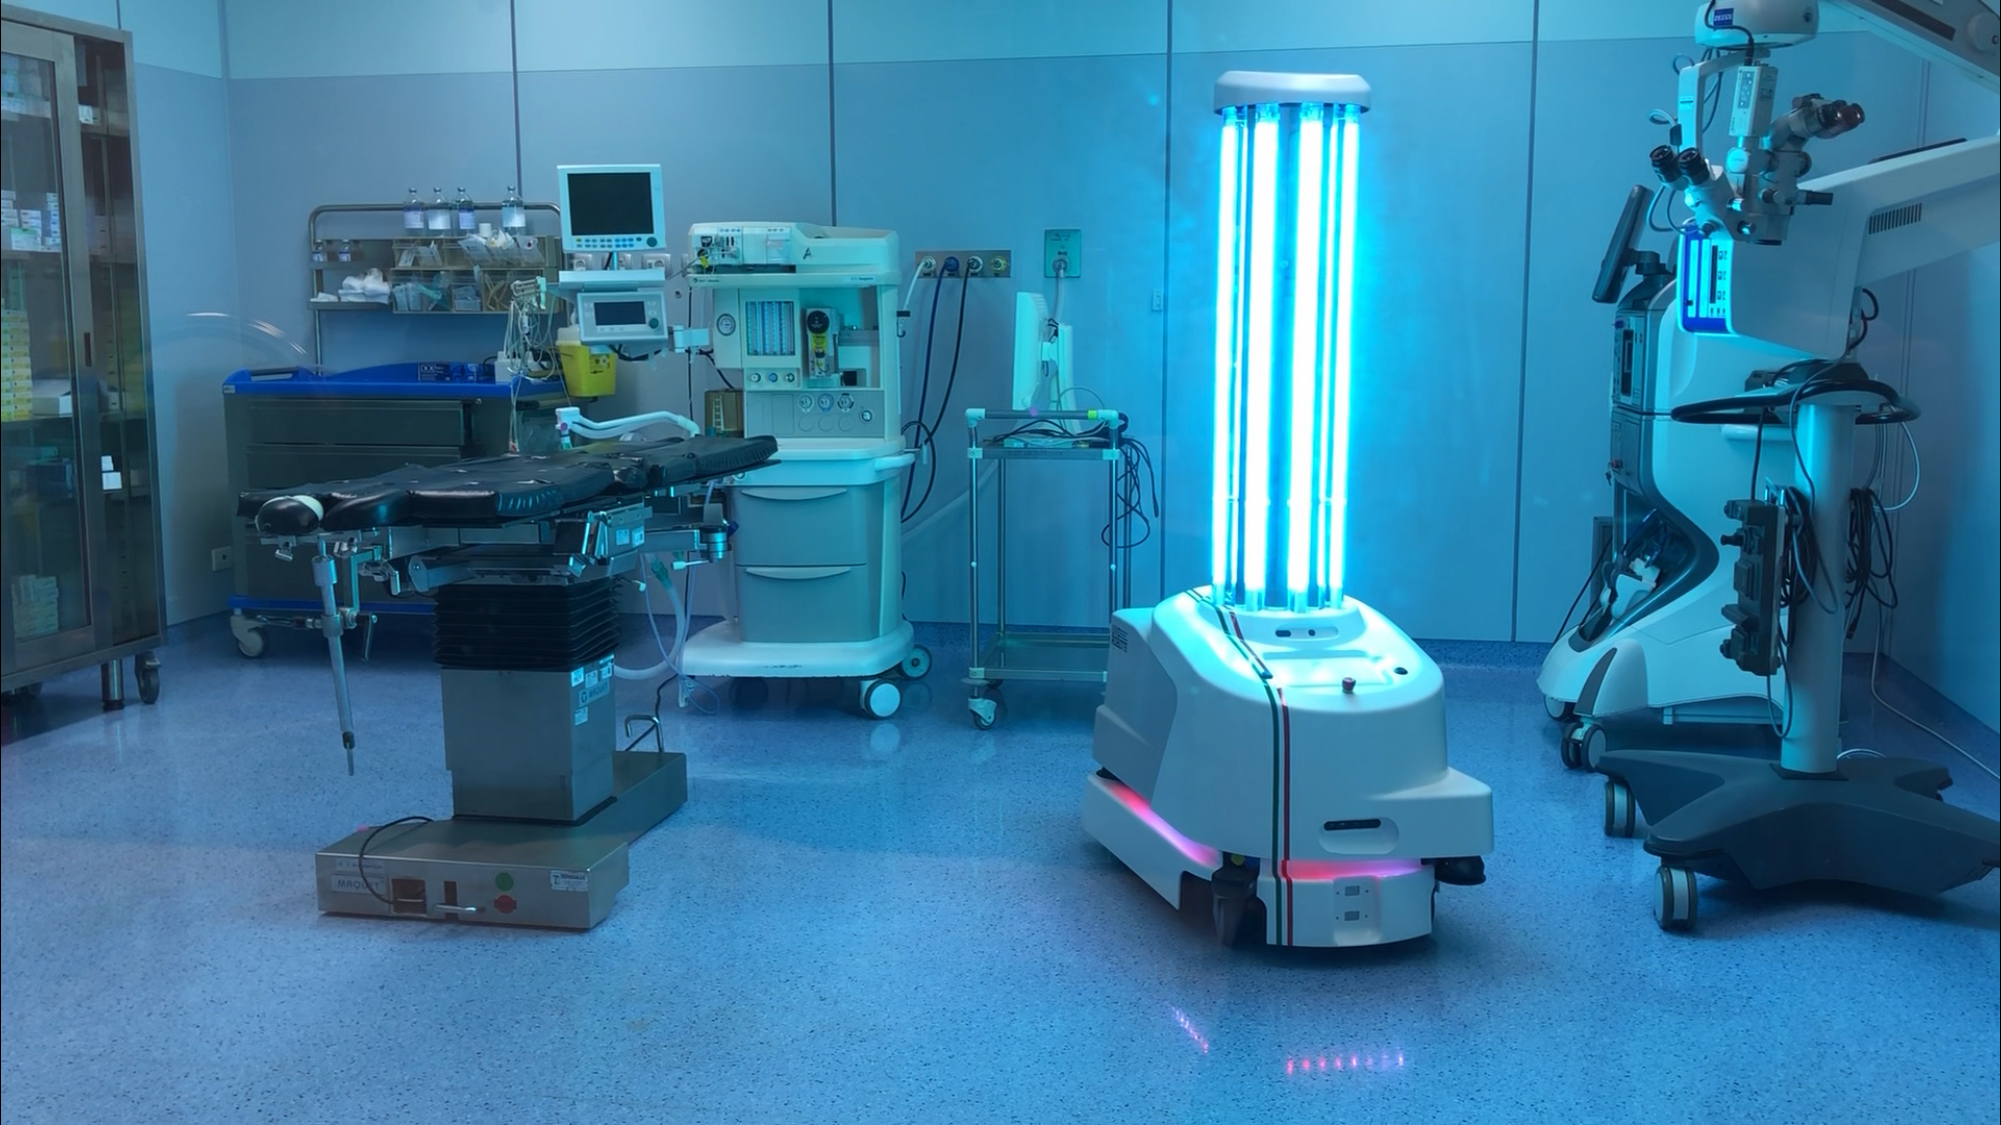
\includegraphics[width=\textwidth,height=2.2 cm]{figs/img/covid.jpg}
      
    \end{subfigure}
    ~ %add desired spacing between images, e. g. ~, \quad, \qquad, \hfill etc. 
      %(or a blank line to force the subfigure onto a new line)
    \begin{subfigure}[b]{0.3\textwidth}
        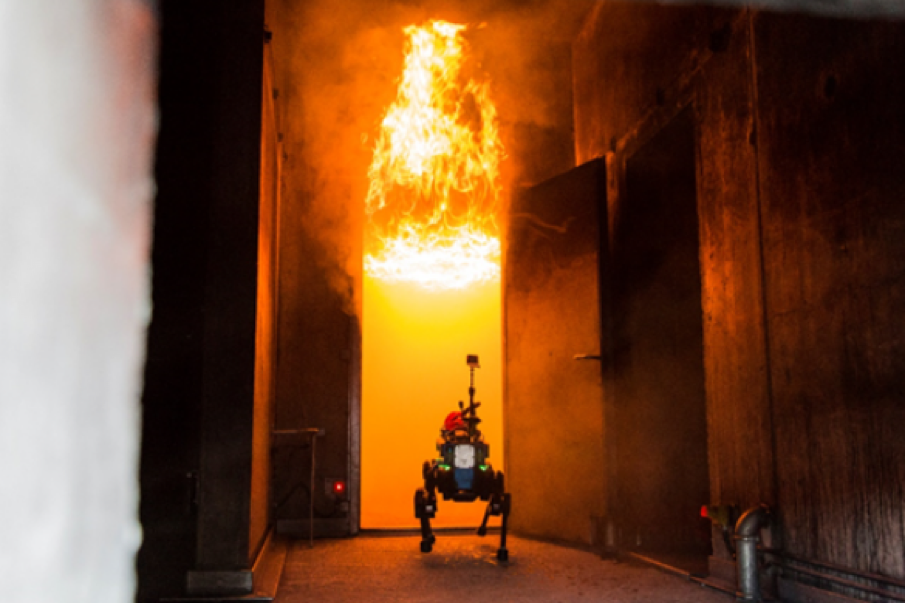
\includegraphics[width=\textwidth]{figs/img/searchRescue.png}
     
    \end{subfigure}
    ~ %add desired spacing between images, e. g. ~, \quad, \qquad, \hfill etc. 
    %(or a blank line to force the subfigure onto a new line)
    \begin{subfigure}[b]{0.3\textwidth}
        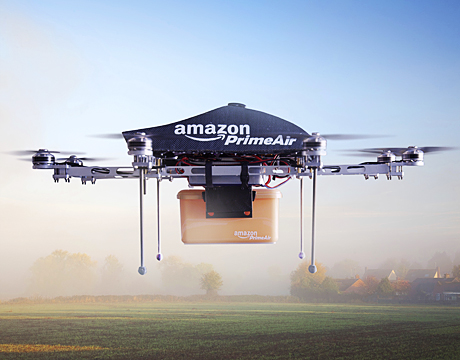
\includegraphics[width=\textwidth,height = 2.2 cm]{figs/img/amazon.jpg}
    
    \end{subfigure}
    \caption{Robots Application}\label{fig:applications}
\end{figure}



Robot Applications in real world:
\begin{itemize}
\item Health Care.
\item  Perimeter surveillance 
\item Environment monitoring 
\item  Cooperative estimation and formation control
\item Indoor navigation using mobile robots.
\end{itemize}
  
\end{frame}

\begin{frame}{Introduction}{Why Dynamic Target Tracking?}
\begin{figure}
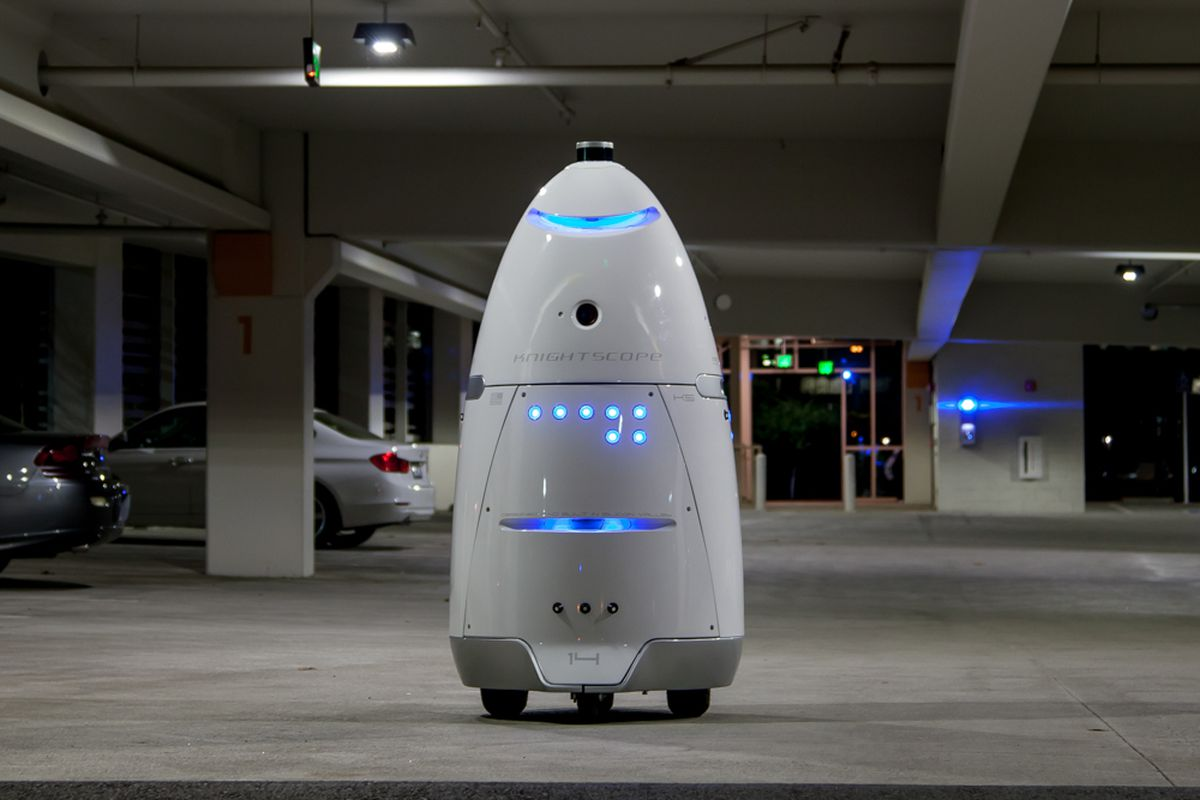
\includegraphics[scale=0.2]{figs/img/security.jpg}
\caption{Security Robot}
\end{figure}
\end{frame}

%%--------------
\section{Problem Setting}
\begin{frame}{What is Dynamic Target Tracking?}
\begin{center}
\begin{figure}
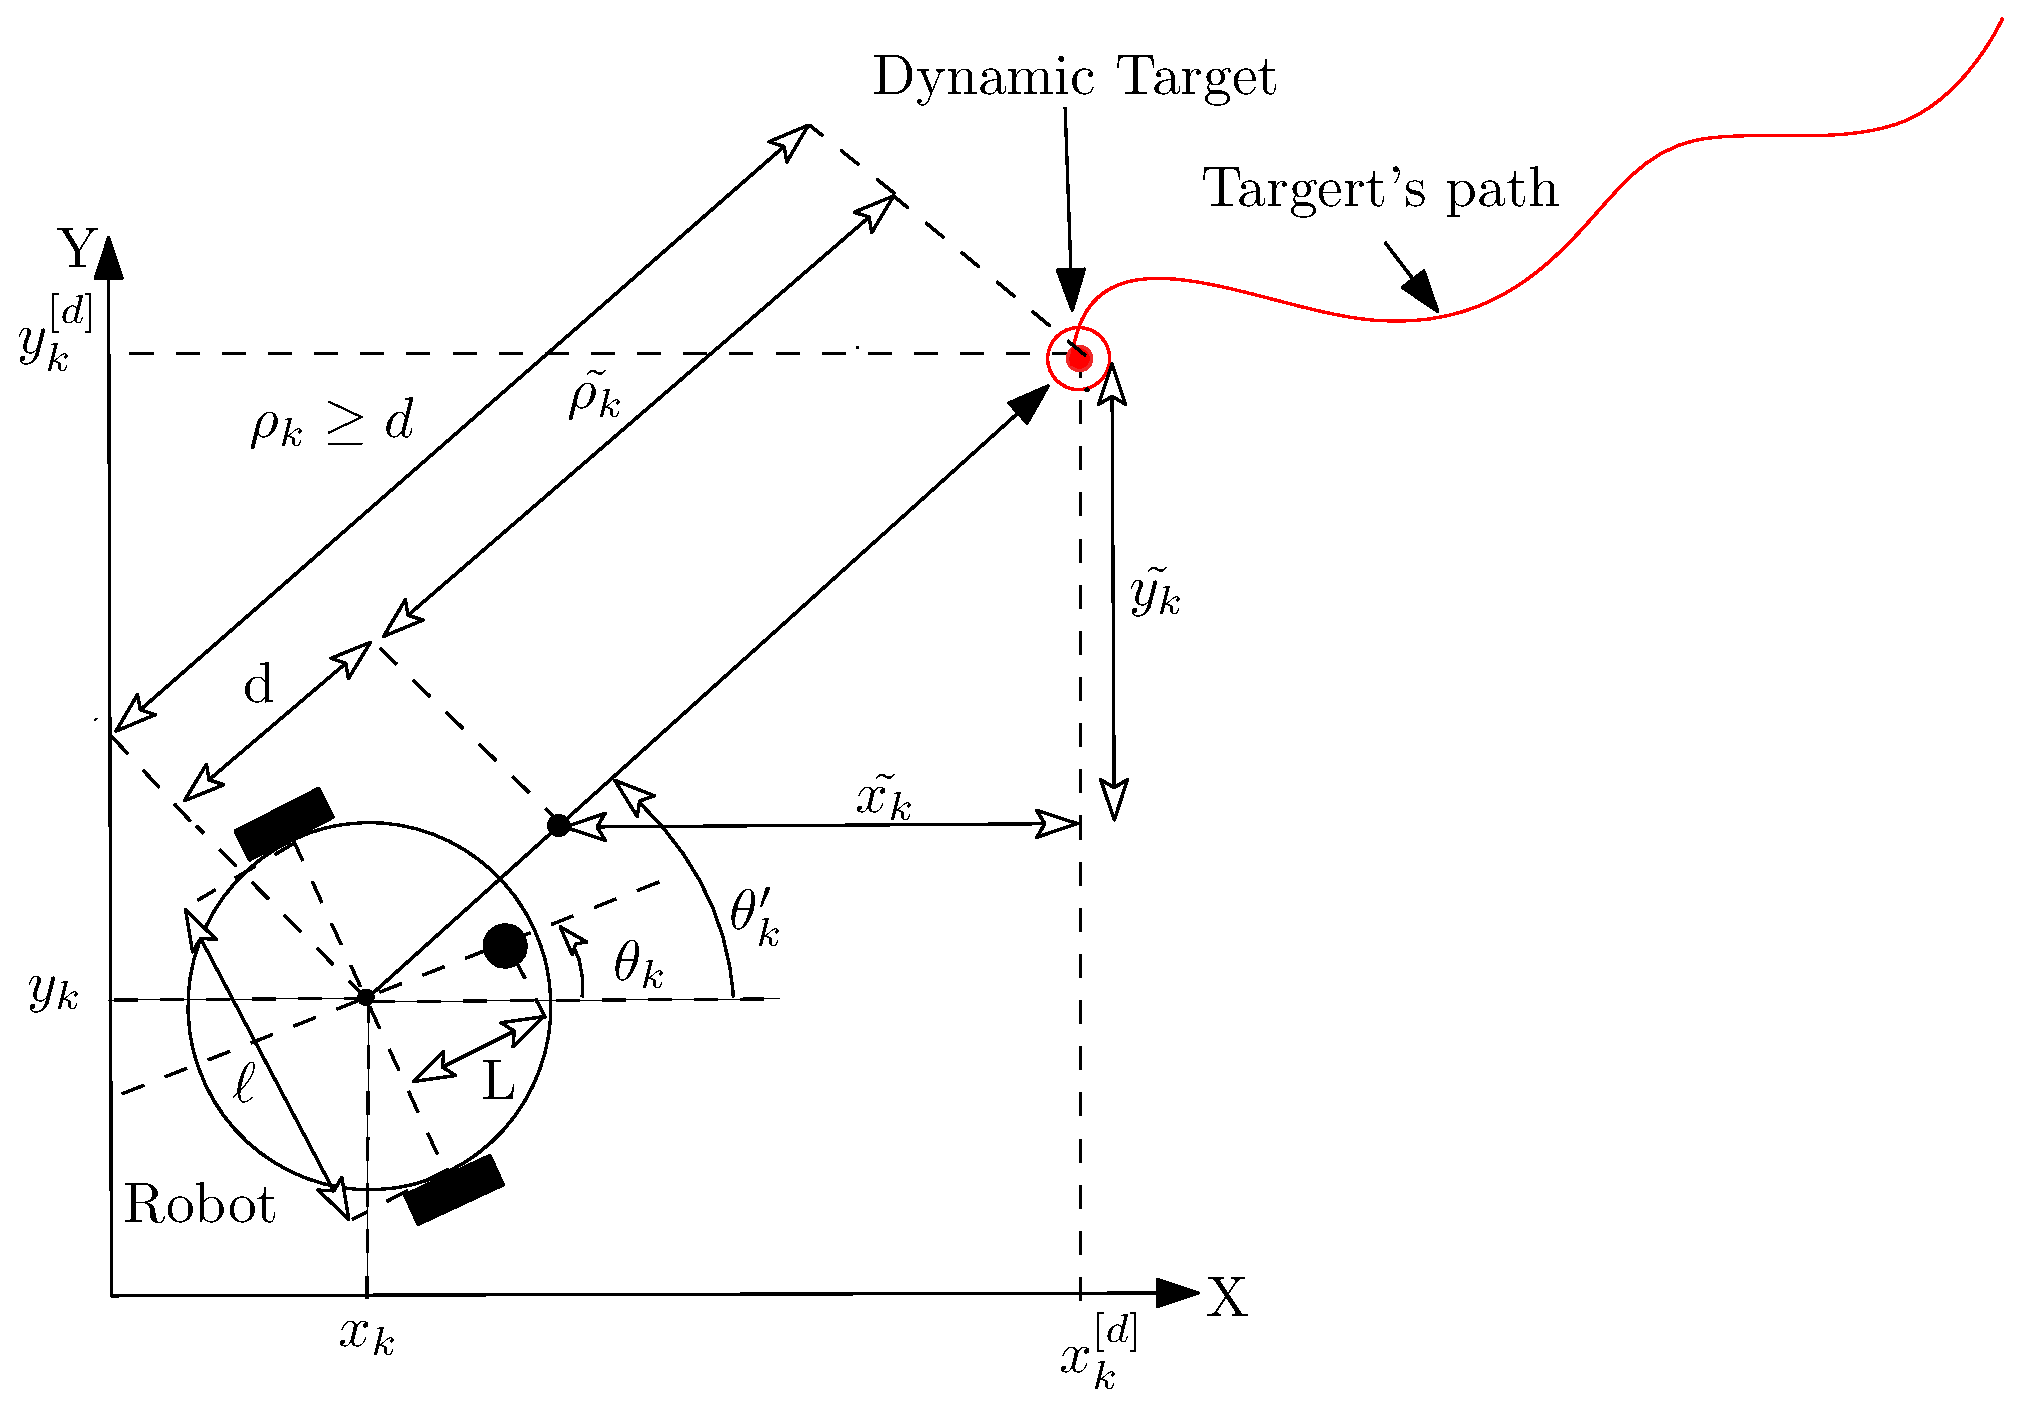
\includegraphics[scale=0.3]{figs/ipe/LFMICSetup.eps}
\caption{problem setting}
\end{figure}
\end{center}
\end{frame}
%

%%------------------------
\section{Previous Approaches}
\begin{frame}{Traditional Approaches}{Litrature Review}
\begin{itemize}
\item The target or it's path is static. 
\item Rely on dynamic models for both the target and the robot.
\end{itemize}
\end{frame}
%-----------------------------
\section{Reinforcement Learning Approach}
\begin{frame}{Our Approach}{What is RL Learning?}
\begin{columns}
\begin{column}{0.5\textwidth}
\begin{itemize}
\item Reinforcement learning (RL) is an emerging sub-field of
machine learning which refers to a set of algorithms and
techniques in which agents learn by interacting with the
environment and determine their own sets of actions that define
trajectories.
\end{itemize}
\end{column}
\begin{column}{0.5\textwidth}
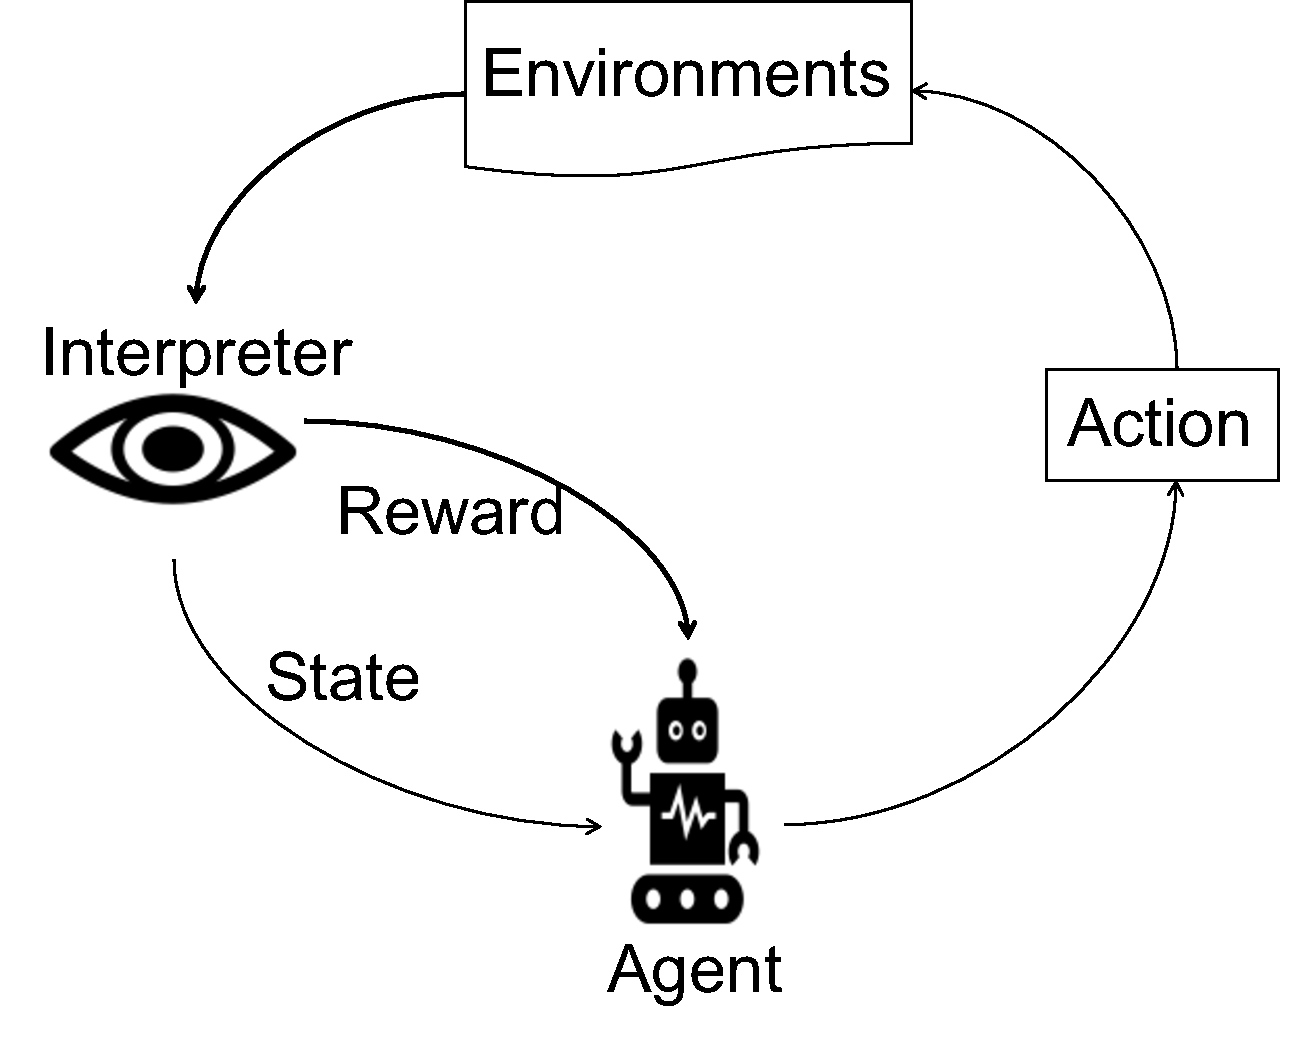
\includegraphics[scale=0.25]{figs/img/Ref-L-agent.pdf}
\end{column}
\end{columns}
\end{frame}
%-----------------------------------
\begin{frame}{Key Equations}
\begin{equation}
  J =  \frac{1}{2} \sum_{k=0}^\infty\left[{\bf e}_k^T \, {\bf Q} \, {\bf e}_k + {\bf u}_k^T \, {\bf R} \, {\bf u_k}\right],
\end{equation}
\begin{equation}
 \mathbf{u}_k^* = -\,  \mathbf{P}_{uu}^{-1}\, \mathbf{P}_{ue}\, \mathbf{e}_k,
\end{equation}
\begin{center}
with P being:
 ${\bf P}=\begin{bmatrix} 
 2\,\omega_c^{[1]}    & \omega_c^{[2]}      & \omega_c^{[3]}       & \omega_c^{[4]}        \\ 
 \omega_c^{[2]}       &2\, \omega_c^{[5]}   & \omega_c^{[6]}       & \omega_c^{[7]}        \\
 \omega_c^{[3]}       & \omega_c^{[6]}      &2\, \omega_c^{[8]}   & \omega_c^{[9]}   \\   
 \omega_c^{[4]}       & \omega_c^{[7]}      & \omega_c^{[9]}      & 2\,\omega_c^{[10]}      
 \end{bmatrix}\in \mathbb{R}^{4\times 4}$
 \end{center}
\end{frame}
%%-------------------------
\section{Computer Simulations}
\begin{frame}{Results}{First Scenario}{Sine wave}
\begin{figure} 
{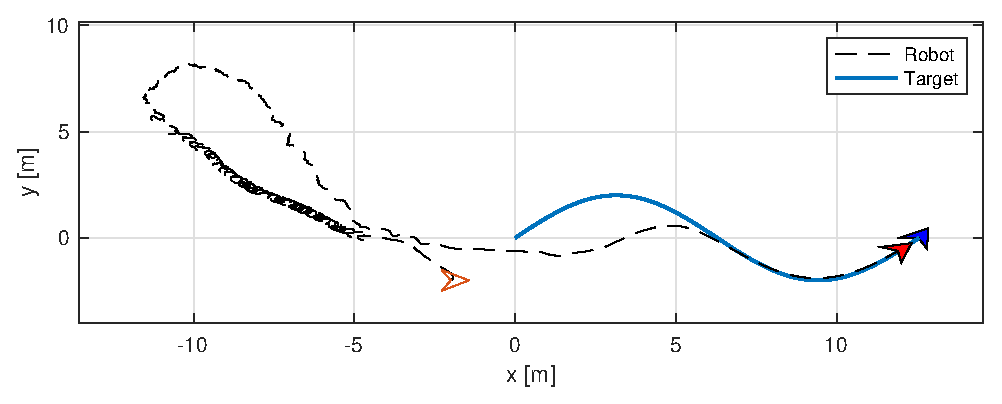
\includegraphics[scale=0.3]{figs/matlab/Sinewave/trajectorySineWave.eps}}
{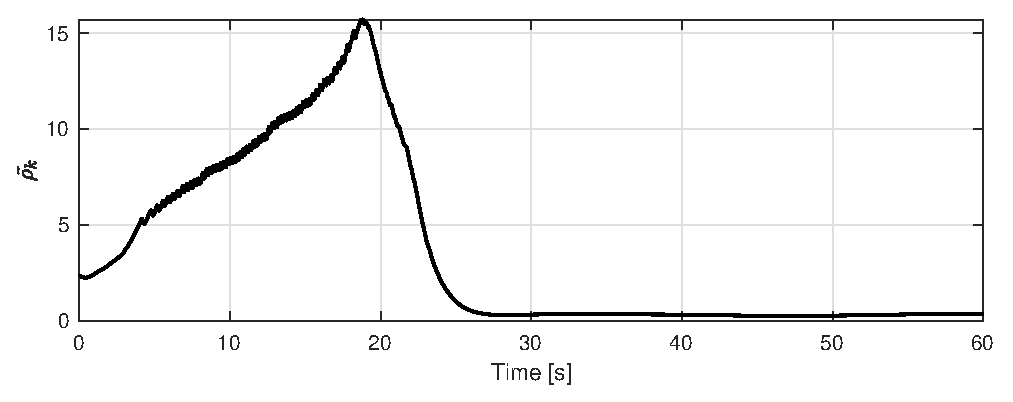
\includegraphics[scale=0.3]{figs/matlab/Sinewave/euclideanDistanceSineWave.eps}}
\caption{Trajectory and Euclidean Distance}
\end{figure}
\begin{figure}
{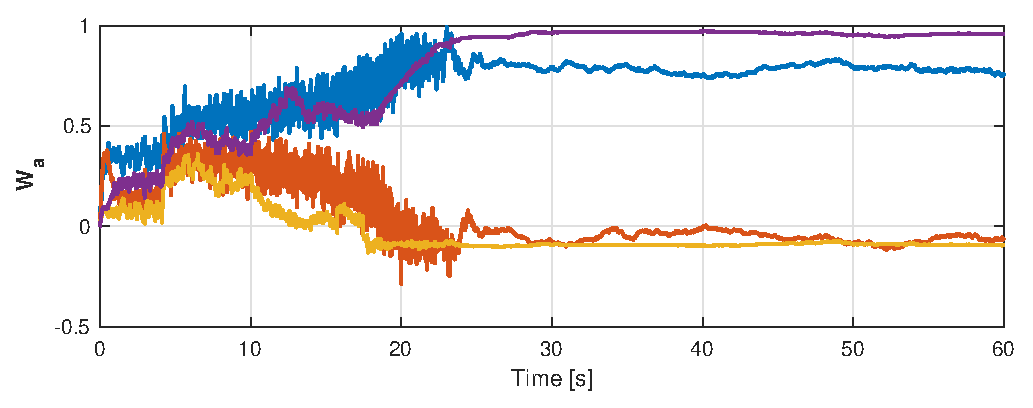
\includegraphics[scale=0.3]{figs/matlab/Sinewave/weightActorSineWave.eps}}
{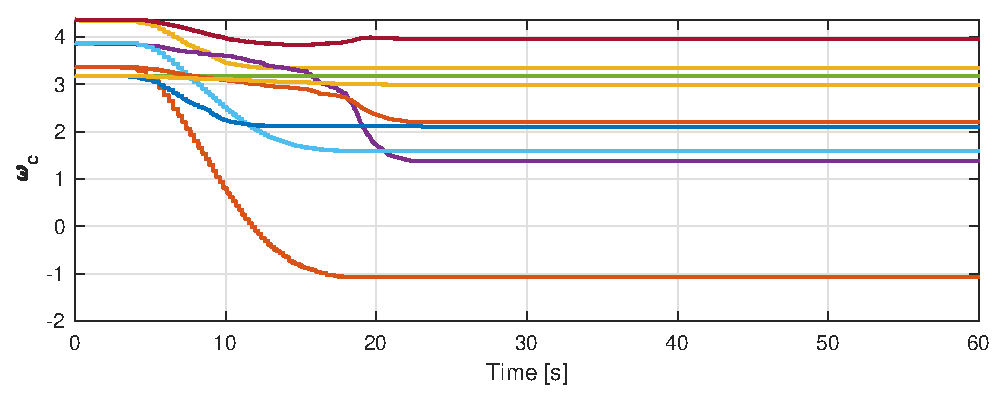
\includegraphics[scale=0.3]{figs/matlab/Sinewave/weightSineWave.eps}}
\caption{Actor and Critic Weights}
\end{figure}
\end{frame}
%%----------------
\begin{frame}{Results}{Second Scenario}{Random Path}
\begin{figure} 
{\includegraphics[scale=0.4]{figs/matlab/Random/trajectoryRandom.eps}}
{\includegraphics[scale=0.4]{figs/matlab/Random/euclideanDistanceRandom.eps}}
\caption{Trajectory and Euclidean Distance}
\end{figure}
\begin{figure}
{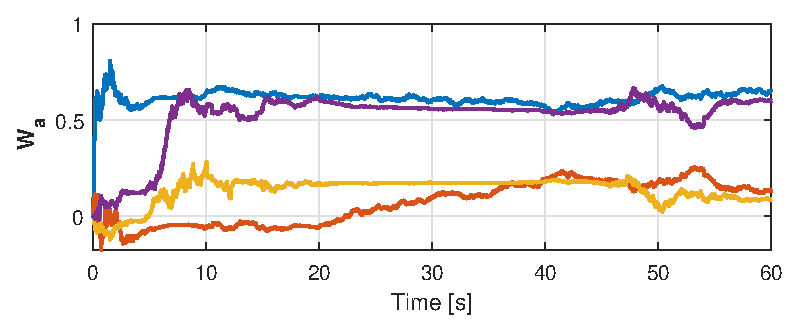
\includegraphics[scale=0.4]{figs/matlab/Random/weightActorRandom.eps}}
{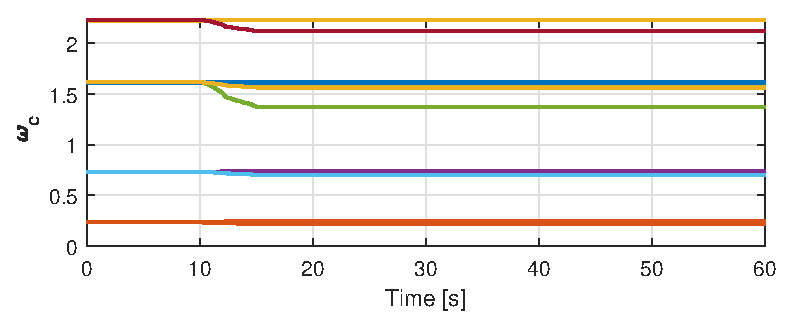
\includegraphics[scale=0.4]{figs/matlab/Random/weightRandom.eps}}
\caption{Actor and Critic Weights}
\end{figure}
\end{frame}
%--------------
\section{Conclusion}
\begin{frame}{In Summary}
\begin{itemize}
\item A model free actor-critic reinforcement learning algorithm for dynamic target
tracking has been proposed and validated using a set of computer experiments .
\item  a differential drive mobile robot and a randomly moving target are
utilized in the simulation. 
\item The actor weights which
drives the control actions of the robot successfully converge to values that
enable the robot to asymptotically track the moving target through unplanned
trajectory. 
\end{itemize}
\end{frame}
%\begin{frame}{Conclusion}
%In this work, we have presented a new framework,
%MAFOSS, that can be used to implement algorithms for multiagent systems. Two different experiments have been conducted
%to show the proposed framework’s ability to conduct motion
%control algorithms using multiple differential-drive mobile
%robots/agents. A potential future work will include testing the
%proposed MAFOSS for implementing more complex multiagent control algorithms, such as area coverage control and
%cooperative estimation while incorporating sensory measurements.
%
%\end{frame}
%--------------------------------------
\section*{Thanks}
\begin{frame}
\begin{LARGE}
\begin{center}
Thanks !
\end{center}
\end{LARGE}
\end{frame}
%-------------------
\end{document}



%%% Local Variables:
%%% mode: latex
%%% TeX-master: t
%%% End:
